\begin{appendices}

	\chapter{Outline Project Specification}
	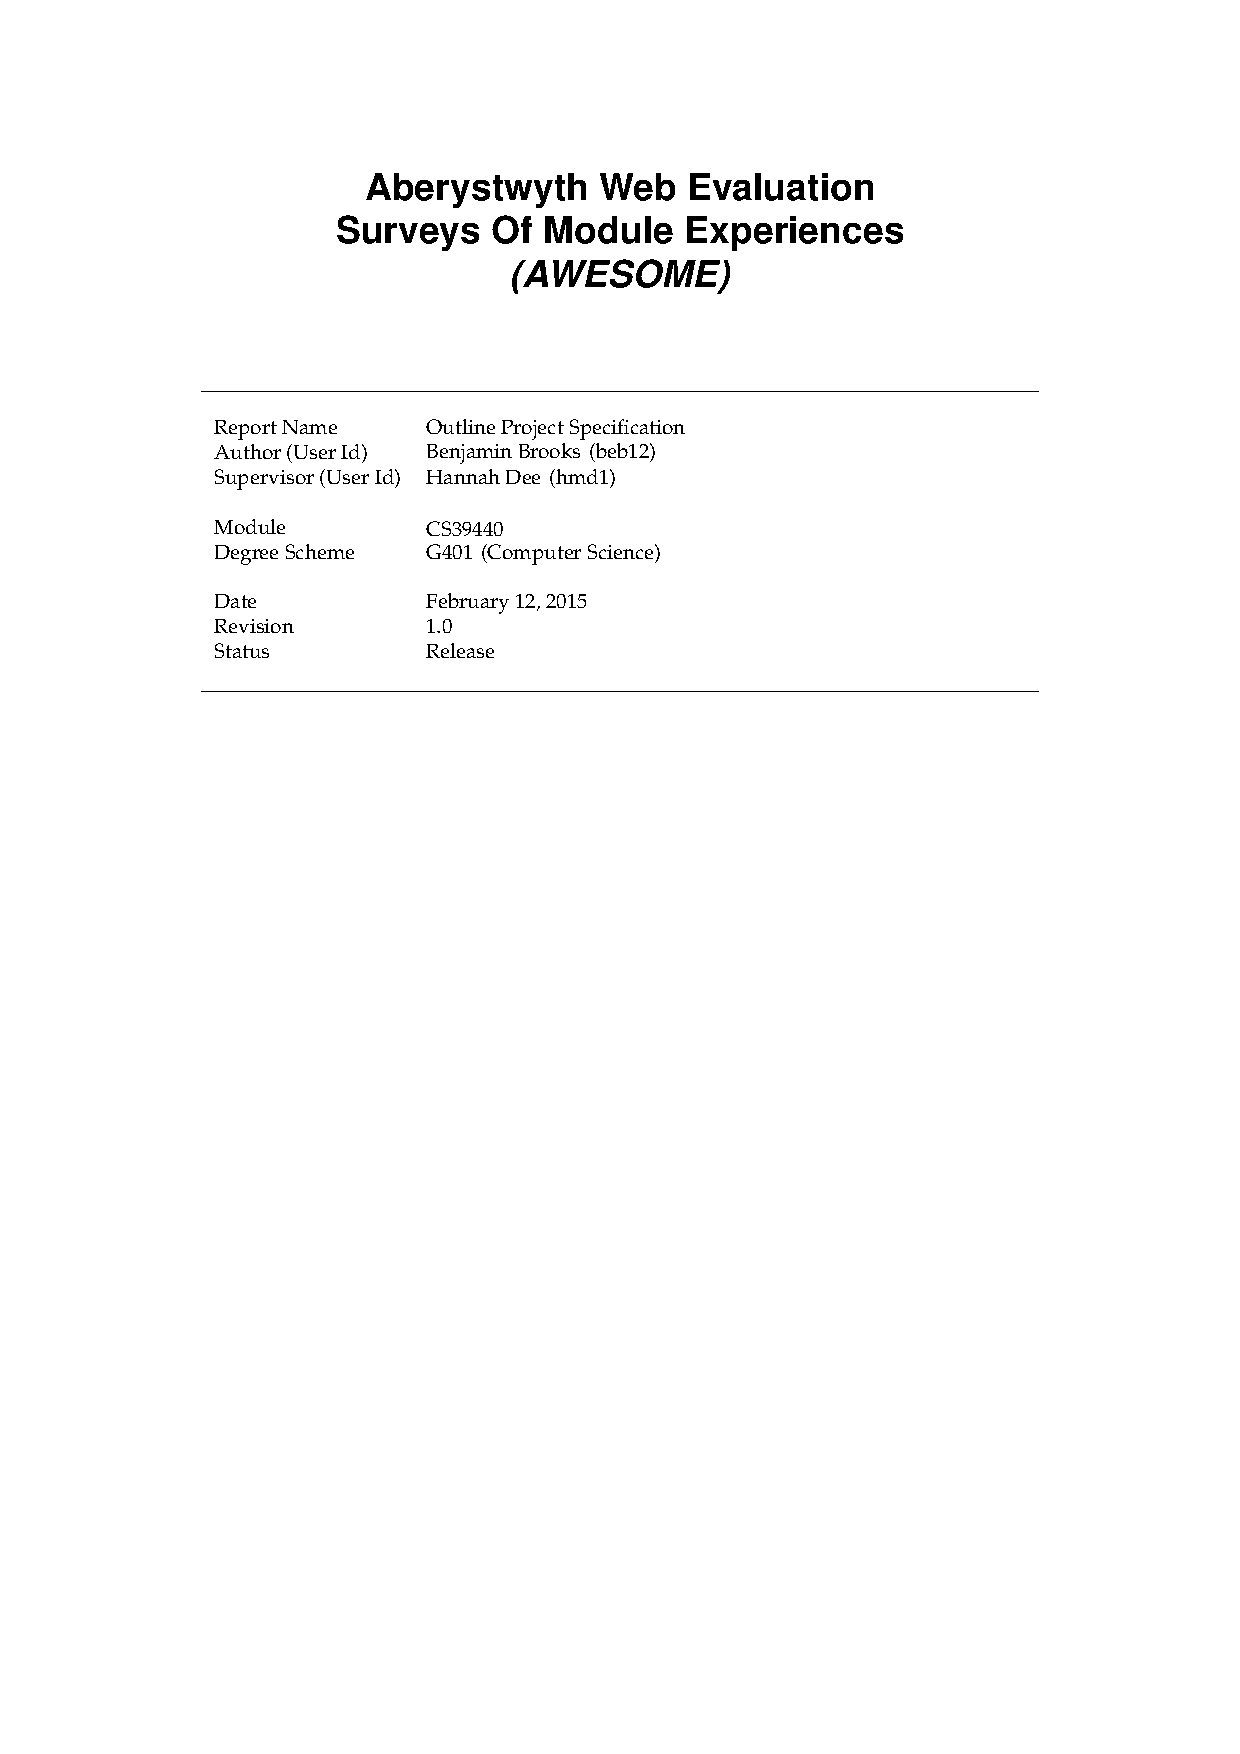
\includepdf[pages=-,scale=.8,pagecommand={}]{../outlinespec/beb12_OutlineProjectSpecification.pdf}


	\chapter{Test Tables}
	\label{app:testtables}
	
	These tests were carried out as part of acceptance testing using the submitted version of \ac{AWESOME}.
	Results are listed below.
	
	\begin{itemize}
		\item Test D8 fails as there is currently no safeguard in place for incorrect \ac{CSV} format.
		\item Test D12 fails as questionnaire respondent tokens aren't created until the moment of sending.
	\end{itemize}
	
	Both of these issues a quick fixes, but are unable to be implemented in time for the dissertation hand-in.
	They will be fixed in a future version.

	\begin{sidewaystable}
		
		\begin{tabularx}{\textwidth}{l|XXXX|r}
			ID &
			Requirement &
			Input &
			Expected Output &
			Actual Output &
			Pass \\
			\midrule
			D1	&	Admin Dashboard sits behind a login	&	Go to \url{awesome.url/admin}	&	Login form pops up	&	Login form pops up	&	\OK \\
			\hline
			D2	&	Admin Dashboard login accepts correct username and password	&	Enter correct credentials into login form	&	Redirected to admin dashboard	&	Redirected to admin dashboard	&	\OK \\
			\hline
			D3	&	Admin Dashboard login refuses incorrect username	&	Enter incorrect username and correct password	&	Login fails	&	Login Fails	&	\OK \\
			\hline
			D4	&	Admin Dashboard login refuses incorrect password	&	Enter correct username and incorrect password	&	Login fails	&	Login Fails	&	\OK \\
			\hline
			D5	&	Create Survey button starts the creation of survey wizard	&	Click `Create Survey' button	&	Taken to screen asking for titles, description, and CSV data	&	Taken to screen asking for titles, description, and CSV data	&	\OK \\
			\hline
			D6	&	Survey must have a title	&	Enter no title and press `create' button	&	Message pops up disallowing action	&	Message pops up disallowing action	&	\OK \\
			\hline
			D7	&	Survey must have CSV data	&	Enter no \ac{CSV} data and press `create' button	&	Message pops up disallowing action	&	Message pops up disallowing action	&	\OK \\
			\hline
			D8	&	Must check CSV data for formatting issues	&	Enter incorrect \ac{CSV} data and press `create' button	&	Message pops up informing of CSV formatting error	&	Taken to survey page without any errors	&	\KO \\
			\hline
			D9	&	Unlocked survey page allows entry of question text and type	&	Type a question title and select an answer type for a question	&	Able to enter text in question text and select an answer type	&	Able to enter text in question text and select an answer type	&	\OK \\
			\hline
			D10	&	Able to add a new question	&	Click add question button	&	A new question text and answer type row appears	&	A new question text and answer type row appears	&	\OK \\
			\hline
			D11	&	Able to delete an existing question	&	Click the delete question button next to a question	&	The question is removed and deleted on save	&	The question is removed and deleted on save	&	\OK \\
			\hline
			D12	&	Be able view participants in a survey before sending	&	Click `Participants' tab in a survey page	&	Respondents should be listed	&	Respondent list is empty	&	\KO \\
			\hline
			D13	&	Be able to send a survey	&	Click the `Send' button in a survey page	&	A message displaying how many people the survey was sent to	&	A message displaying how many people the survey was sent to	&	\OK \\
			\bottomrule
		\end{tabularx}
	
		\caption{Acceptance testing table of \acs{AWESOME}'s Admin Dashboard}
		\label{tbl:awesomeacceptancetestingdashboard}
		
	\end{sidewaystable}

	\begin{sidewaystable}
		
		\begin{tabularx}{\textwidth}{l|XXXX|r}
			ID &
			Requirement &
			Input &
			Expected Output &
			Actual Output &
			Pass \\
			\midrule
			Q1	&	Students receive an email with a link to personalised questionnaire	&	Check email inbox	&	See an email with unique link	&	See an email with unique link	&	\OK \\
			\hline
			Q2	&	Questionnaire can be viewed correctly	&	Click link in email	&	See questionnaire displayed	&	See questionnaire displayed	&	\OK \\
			\hline
			Q3	&	Answers can be selected or filled in	&	Click on a Likert rating or type in a text box	&	See answer selected or text typed in	&	See answer selected or text typed in	&	\OK \\
			\hline
			Q4	&	Answers can be submitted	&	Select or type some answers and press the send button	&	Page redirected with a message informing of completion	&	Page redirected with a message informing of completion	&	\OK \\
			\hline
			Q5	&	Questionnaire can't be completed twice	&	Re-visit the unique link and try to complete the survey again	&	Receive an error message informing that the questionnaire has already been completed	&	Receive an error message informing that the questionnaire has already been completed	&	\OK \\
			\bottomrule
		\end{tabularx}
			
		\caption{Acceptance testing of \acs{AWESOME}'s Questionnaire}
		\label{tbl:awesomeacceptancetestingquestionnaire}
		
	\end{sidewaystable}
	
\end{appendices}
